% ---
% Capitulo de Materiais e Metodos
% ---

\chapter{Materiais e Métodos\label{cha:methods}}

Este capítulo especifica o método proposto e o protocolo experimental usado para avaliá-lo. A Seção \ref{sec:overview} apresenta a visão geral da construção. A Seção \ref{sec:notation} fixa a notação. As Seções \ref{sec:knn} e \ref{sec:bridges} detalham, respectivamente, a construção decomposta do grafo de vizinhança e a estimativa que substitui a árvore geradora. A Seção \ref{sec:algorithm} reúne o método em pseudocódigo. A Seção \ref{sec:implementation} descreve a implementação e o esquema de execução em múltiplos aceleradores. A Seção \ref{sec:protocol} especifica o protocolo experimental, incluindo as referências exatas contra as quais a qualidade é medida, as métricas, os conjuntos de dados e as linhas de base.

% =====================================================================
\section{Visão geral do método\label{sec:overview}}
% =====================================================================

A Figura \ref{fig:pipeline} descreve o fluxo de uma construção. O conjunto de dados atravessa quatro etapas.\\

Na primeira, os pontos são particionados em $m$ instâncias. Uma permutação aleatória do conjunto é cortada em $m$ blocos, e cada bloco, acrescido de uma amostra de sobreposição sorteada dos demais blocos, forma uma instância. Cada instância é um problema completo de NN-Descent sobre os seus próprios pontos e é executada em qualquer acelerador disponível.\\

Na segunda, as vizinhanças produzidas pelas instâncias são mescladas nas listas globais dos $\kmax$ melhores. Como o particionamento deixa não comparado todo par cujos pontos caiam em blocos distintos, um passo de reparo sobre o grafo mesclado se segue à mesclagem.\\

Na terceira, o índice de \textit{hubness} é calculado e os candidatos a anti-hub são selecionados; a quantidade de candidatos é $\lceil d \ln |E| \rceil$, onde $d$ é a dimensionalidade adotada para o conjunto de dados e $|E|$ é o número de arestas não direcionadas do \ac{k-NNG}.\\

Na quarta, uma árvore geradora é calculada sobre os anti-hubs selecionados, produzindo as arestas de ponte, seguida de uma etapa de reparo de conectividade que liga quaisquer componentes que as pontes tenham deixado separados, de modo que o resultado seja sempre uma árvore geradora e não uma floresta.\\

Concluída a construção, uma consulta pela $\mathrm{MST}_{\mpts}$ repesa a união das arestas do \ac{k-NNG} com as arestas de ponte usando $\mrd^{\mpts}$ e extrai uma árvore geradora de $O(n\kmax)$ arestas.\\

\begin{figure}[htb!]
\centering
\caption{\label{fig:pipeline} O fluxo de uma construção. As instâncias são subproblemas independentes e constituem a unidade de paralelismo. A mesclagem, o passo de reparo e a árvore geradora das pontes são globais; as duas primeiras operam sobre o grafo inteiro e executam na \ac{CPU}, e a terceira opera sobre um conjunto de $\lceil d\ln|E|\rceil$ vértices, muito menor que o conjunto de dados.}
\begin{tikzpicture}[
  node distance=4mm,
  box/.style={draw, rounded corners=1pt, align=center, font=\scriptsize,
              minimum height=7mm, inner xsep=2pt, text width=33mm},
  wide/.style={box, text width=105mm},
  ar/.style={-{Latex[length=1.6mm]}, thin}
]
\node[wide, fill=black!5] (data) {conjunto de dados $X$, $|X| = n$};
\node[wide, below=of data] (part) {particionamento em $m$ blocos\\{\tiny cada bloco $B_i$ recebe uma amostra de sobreposição $S_i$ dos demais}};
\node[box, below=of part.south west, anchor=north west] (i1) {instância 1\\{\tiny $B_1 \cup S_1$}};
\node[box, right=3mm of i1] (i2) {instância 2\\{\tiny $B_2 \cup S_2$}};
\node[box, right=3mm of i2] (i3) {instância $m$\\{\tiny $B_m \cup S_m$}};
\node[wide, below=of i2] (merge) {mesclagem nas listas globais de $\kmax$ melhores};
\node[wide, below=of merge] (refine) {passo de reparo: NN-Descent sobre o grafo mesclado};
\node[wide, below=of refine, fill=black!5] (knn) {grafo de $\kmax$ vizinhos mais próximos};
\node[wide, below=of knn] (hub) {índice de \textit{hubness}: graus reversos, pontuação local,\\seleção de $\lceil d\ln|E|\rceil$ anti-hubs};
\node[wide, below=of hub] (br) {árvore geradora sobre os anti-hubs $+$ reparo de conectividade};
\node[wide, below=of br, fill=black!5] (sg) {CORE-SG $=$ $k$-NNG $\cup$ pontes};
\node[wide, below=of sg] (out) {$\mathrm{MST}_{\mpts}$ para qualquer $\mpts \le \kmax$\\{\tiny repesar com $\mrd^{\mpts}$, depois extrair a MST}};

\draw[ar] (data) -- (part);
\draw[ar] (part.south) -- ++(0,-1.4mm) -| (i1.north);
\draw[ar] (part.south) -- ++(0,-1.4mm) -| (i2.north);
\draw[ar] (part.south) -- ++(0,-1.4mm) -| (i3.north);
\draw[ar] (i1.south) |- ([yshift=1.4mm]merge.north);
\draw[ar] (i2.south) -- (merge.north);
\draw[ar] (i3.south) |- ([yshift=1.4mm]merge.north);
\draw[ar] (merge) -- (refine);
\draw[ar] (refine) -- (knn);
\draw[ar] (knn) -- (hub);
\draw[ar] (hub) -- (br);
\draw[ar] (br) -- (sg);
\draw[ar] (knn.east) -- ++(4mm,0) |- (sg.east);
\draw[ar] (sg) -- (out);
\end{tikzpicture}\\
Fonte: Autoral.
\end{figure}

% =====================================================================
\section{Notação\label{sec:notation}}
% =====================================================================

Seja $X \subset \mathbb{R}^d$ um conjunto de $n$ pontos de dimensionalidade ambiente $d$, e seja $d(\cdot,\cdot)$ uma medida de distância sobre ele. Seguindo a convenção da literatura de agrupamento baseado em densidade, o símbolo $d$ é usado com dois sentidos: isolado, denota a dimensionalidade ambiente, que é um número; acompanhado de dois argumentos, denota a medida de distância. Os dois usos se distinguem sem ambiguidade pela presença dos argumentos.\\

As definições de \textit{core distance} e \textit{mutual reachability distance} são as das equações \eqref{eq:coredist} e \eqref{eq:mrd}. O parâmetro $\kmax$ é o maior valor de $\mpts$ que o grafo deve servir, e $k$ denota o número de vizinhos armazenados por vértice, que neste trabalho é igual a $\kmax$.\\

Denota-se por $m$ a quantidade de instâncias em que a construção é decomposta; por $B_i$ o bloco de pontos da instância $i$; por $\omega$ a fração de sobreposição, isto é, quantos pontos adicionais cada instância recebe em proporção ao seu próprio bloco; por $\mathrm{NN}(v)$ a lista de vizinhos armazenada para o vértice $v$; e por $|E|$ o número de arestas não direcionadas do \ac{k-NNG} resultante.\\

% =====================================================================
\section{O grafo de vizinhança: instâncias independentes\label{sec:knn}}
% =====================================================================

\subsection{A instância\label{sec:instance}}

Uma instância é a unidade de decomposição da construção. Ela reúne um bloco de pontos, uma amostra de sobreposição extraída dos demais blocos, e as listas de vizinhança desses pontos, e constitui um problema completo de NN-Descent sem referência a estado global.\\

A construção parte de uma permutação aleatória de $X$, cortada em $m$ blocos $B_1, \dots, B_m$ de tamanho aproximadamente $n/m$. A permutação é necessária: cortar o conjunto na ordem em que ele é lido produziria blocos correlacionados com a ordem de armazenamento, que em conjuntos reais frequentemente reflete alguma estrutura, e isso tornaria os resultados dependentes de uma propriedade acidental do arquivo.\\

Três consequências decorrem dessa construção, e são elas que respondem ao problema da Seção \ref{sec:problem-scale}. A memória que uma instância exige é determinada pelo seu próprio tamanho, independentemente do tamanho do conjunto de dados, de modo que um grafo maior do que a memória de um acelerador é processado elevando-se $m$. As instâncias não se comunicam entre si durante a execução e podem portanto ser enfileiradas em qualquer dispositivo livre. E a quantidade de instâncias define a unidade de paralelismo disponível, independentemente de quantos dispositivos a executem; manter $m$ maior ou igual à quantidade de dispositivos é o que mantém todos ocupados.\\

\subsection{A sobreposição\label{sec:overlap}}

Blocos disjuntos deixam não comparado todo par cujos dois pontos caiam em blocos distintos, e deixam também as instâncias sem referência comum: dois blocos só concordariam entre si através dos pontos que ambos por acaso contivessem, o que em uma partição disjunta é nenhum.\\

Cada instância recebe, por isso, além do seu bloco $B_i$, uma amostra $S_i$ de $\omega|B_i|$ pontos sorteados uniformemente entre os demais blocos. O tamanho da instância é, portanto,
\begin{equation}
\label{eq:instancesize}
m_i = (1 + \omega)\,\frac{n}{m},
\end{equation}
antes de removidos os sorteios repetidos.\\

A sobreposição tem dois efeitos, e ambos importam. O primeiro é dar às instâncias um conjunto de referência compartilhado, de modo que vizinhanças descobertas em instâncias distintas possam ser confrontadas na mesclagem. O segundo é que parte dos pares que cruzariam fronteiras passa a ser comparada dentro das instâncias, antes da mesclagem, o que reduz o trabalho que resta ao passo de reparo.\\

Esse segundo efeito é o que torna $\omega$ um parâmetro de projeto, acima de um detalhe de implementação. A fase de instâncias executa nos aceleradores; o passo de reparo não. Elevar $\omega$ aumenta a primeira e reduz o segundo, isto é, desloca trabalho da \ac{CPU} para os dispositivos, ao custo de ocupar mais memória por instância. A Seção \ref{sec:res-overlap} caracteriza esse compromisso, e mostra em particular que elevar $m$ e $\omega$ conjuntamente mantém a residência por dispositivo aproximadamente constante enquanto melhora simultaneamente a qualidade e a escalabilidade.\\

\subsection{A restrição de parada\label{sec:constraints}}

A descida dentro de uma instância termina quando uma rodada produz menos de $\delta k m_i$ atualizações, onde $m_i$ é o tamanho da instância. O critério é expresso em função do tamanho da instância, independentemente do conjunto de dados, o que o mantém atrelado ao subproblema: um critério expresso como fração de $n$ faria instâncias pequenas pararem cedo demais ou tarde demais conforme $m$ variasse.\\

\subsection{O custo de memória por dispositivo\label{sec:devicecost}}

O custo por ponto que uma instância impõe ao dispositivo é
\begin{equation}
\label{eq:devicecost}
c = 4\,\mathrm{stride} + 8k + s,
\end{equation}
em que $\mathrm{stride}$ é o comprimento do vetor após alinhamento, $k$ é o tamanho da vizinhança e $s$ é o estado de amostragem do NN-Descent. Uma instância ocupa, portanto, $c\,m_i$ bytes, com $m_i$ dado pela Equação \eqref{eq:instancesize}, e é a maior instância que decide se uma configuração cabe em um dado acelerador.\\

Duas convenções de unidade são usadas ao longo do texto, e a distinção importa porque os limites derivados desta equação dependem dela. As capacidades de dispositivo seguem a rotulação do fabricante, em múltiplos binários, de modo que um acelerador de 8\,GB oferece $2^{33} = 8{,}59 \times 10^9$ bytes. As quantidades medidas e reportadas, como as residências da Seção \ref{sec:res-memory}, estão em múltiplos decimais de $10^6$ e $10^9$ bytes.\\

Essa expressão é a resposta operacional ao problema da Seção \ref{sec:problem-scale}. Dada a memória disponível em um dispositivo, os pares $(m, \omega)$ que cabem nele são calculáveis, e não precisam ser descobertos por tentativa. A Seção \ref{sec:res-memory} reporta a grandeza diretamente medida.\\

\subsection{Mesclagem\label{sec:merge}}

Concluídas as instâncias, suas vizinhanças são mescladas no grafo global por inserção repetida em listas ordenadas dos $\kmax$ melhores: cada instância oferece as vizinhanças que descobriu, e cada candidato é aceito apenas se melhorar a lista em que é oferecido.\\

Essa operação é comutativa e associativa, o que significa que o resultado mesclado não depende da ordem em que as instâncias terminam nem de como seus resultados são agrupados, e é idempotente, o que significa que mesclar a mesma vizinhança duas vezes não altera nada. As instâncias podem, portanto, terminar em qualquer ordem, e o escalonador não precisa de nenhum protocolo de coordenação além de recolher os resultados.\\

Como as instâncias se sobrepõem, um mesmo vértice pode receber contribuições de mais de uma delas, e a mesclagem é o ponto em que essas contribuições são confrontadas. É essa propriedade que faz da sobreposição um mecanismo útil em vez de um desperdício de trabalho duplicado.\\

\subsection{O passo de reparo\label{sec:repair-pass}}

O particionamento deixa não comparado todo par cujos pontos não compartilhem nenhuma instância, de modo que o grafo mesclado omite vizinhos que uma descida única e indivisa teria encontrado. Um passo de reparo, que é uma nova execução de NN-Descent sobre o grafo mesclado, os recupera.\\

Esse passo existe exclusivamente como consequência do particionamento: em $m = 1$ o resultado da descida é adotado diretamente e nenhum reparo é executado. Ele opera sobre o grafo inteiro e é, por isso, global no sentido da Seção \ref{sec:asymmetry}; ele executa na \ac{CPU}, e é a fase que não escala com a quantidade de aceleradores.\\

O passo de reparo é a fase dominante de uma construção em escala, e por isso recebeu atenção específica. Nenhuma das quatro estratégias de redução da Seção \ref{sec:discarded-repair} o encurtou a qualidade constante. O que o reduz é a sobreposição da Seção \ref{sec:overlap}, que não o encurta mas desloca parte de seu trabalho para as instâncias. A Seção \ref{sec:res-repair} reporta as medições correspondentes.\\

% =====================================================================
\section{A árvore geradora: pontes anti-hub\label{sec:bridges}}
% =====================================================================

\subsection{O estimador de borda\label{sec:score}}

Como estabelecido na Seção \ref{sec:adopted-bridges}, a árvore geradora só precisa fornecer arestas que atravessem componentes separados por densidade, e tal ponte parte da borda de um componente. Define-se, para um vértice $v$ do \ac{k-NNG} com conjunto de vizinhos $\mathrm{NN}(v)$,
\begin{equation}
\label{eq:rd}
\mathrm{rd}(v) = \left| \{\, u : v \in \mathrm{NN}(u) \,\} \right|,
\end{equation}
o grau reverso, isto é, o número de vértices que listam $v$ entre seus próprios $k$ vizinhos mais próximos, e
\begin{equation}
\label{eq:score}
\mathrm{score}(v) = \frac{\mathrm{rd}(v)}
     {\dfrac{1}{|\mathrm{NN}(v)|}\displaystyle\sum_{u \in \mathrm{NN}(v)} \mathrm{rd}(u)},
\end{equation}
o grau reverso de $v$ dividido pelo grau reverso médio sobre os próprios vizinhos de $v$.\\

Um ponto interior está dentro de muitas das vizinhanças de seus vizinhos; um ponto de borda está dentro de poucas, porque as listas de seus vizinhos apontam de volta para dentro do componente. O denominador é o que torna \eqref{eq:score} utilizável: comparar $\mathrm{rd}(v)$ contra a população global apenas encontraria os componentes esparsos, ao passo que compará-lo contra a própria vizinhança de $v$ torna a pontuação invariante à densidade local. Um ponto de borda de um componente denso pontua como um ponto de borda de um componente esparso, o que é necessário quando os dados misturam densidades. Valores abaixo de 1 indicam um anti-hub local.\\

A Figura \ref{fig:antihub} ilustra os dois mecanismos. O painel (a) mostra a assimetria que o numerador captura: um vértice interior é apontado por muitos de seus vizinhos, um vértice de borda por poucos. O painel (b) mostra por que o denominador é indispensável. Uma ordenação pelo grau reverso bruto colocaria todos os vértices do componente esparso à frente da borda do componente denso, e o orçamento de seleção seria consumido por um único componente; a normalização local desloca ambas as bordas para valores abaixo de 1 e ambos os interiores para valores próximos de 1, de modo que a ordenação passa a separar bordas de interiores em vez de separar componentes densos de esparsos.\\

\begin{figure}[htb!]
\centering
\caption{\label{fig:antihub} O estimador de borda de \eqref{eq:score}. Em (a), arestas direcionadas do \ac{k-NNG} apontando para um vértice interior $v$ e para um vértice de borda $u$: o interior está na lista de vizinhos de muitos, a borda na de poucos. Em (b), dois componentes de densidades distintas, com o grau reverso $\mathrm{rd}$ e a pontuação de \eqref{eq:score} anotados; o grau reverso bruto ordena por densidade, a pontuação normalizada ordena por posição no componente.}
\begin{tikzpicture}[
  pt/.style={circle, draw=black!55, fill=black!12, inner sep=0pt, minimum size=3.4pt},
  hi/.style={circle, draw=black, fill=black, inner sep=0pt, minimum size=5pt},
  ar/.style={-{Latex[length=1.3mm]}, black!50, semithick},
  lb/.style={font=\scriptsize},
  cp/.style={font=\scriptsize}
]
% ---------- painel (a) ----------
\begin{scope}
  \node[pt] (a1)  at (-1.30, 0.70) {};
  \node[pt] (a2)  at (-0.70, 1.15) {};
  \node[pt] (a3)  at ( 0.05, 1.30) {};
  \node[pt] (a4)  at ( 0.75, 1.00) {};
  \node[pt] (a5)  at ( 1.35, 0.62) {};
  \node[pt] (a6)  at (-1.55, 0.05) {};
  \node[pt] (a7)  at (-0.65, 0.35) {};
  \node[hi] (v)   at ( 0.00, 0.00) {};
  \node[pt] (a9)  at ( 0.65, 0.25) {};
  \node[hi] (u)   at ( 1.85, 0.30) {};
  \node[pt] (a11) at (-1.30,-0.65) {};
  \node[pt] (a12) at (-0.65,-1.05) {};
  \node[pt] (a13) at ( 0.10,-1.25) {};
  \node[pt] (a14) at ( 0.85,-0.95) {};
  \node[pt] (a15) at ( 1.45,-0.55) {};
  \foreach \s in {a7,a9,a3,a13,a2,a14} \draw[ar] (\s) -- (v);
  \draw[ar] (a5) -- (u);
  \node[lb, anchor=east] at (-0.12, 0.16) {$v$};
  \node[lb, anchor=west] at ( 1.98, 0.30) {$u$};
  \node[lb, anchor=north] at (0.0,-1.55) {$\mathrm{rd}(v) = 6$ \quad $\mathrm{rd}(u) = 1$};
  \node[cp, anchor=north] at (0.15,-2.00) {(a) interior contra borda};
\end{scope}
% ---------- painel (b) ----------
\begin{scope}[xshift=6.4cm]
  % componente denso
  \foreach \x/\y in {-0.9/0.55, -0.55/0.85, -0.2/0.6, -0.75/0.2, -0.4/0.35,
                     -0.05/0.15, -0.95/-0.2, -0.55/-0.15, -0.2/-0.35,
                     -0.8/-0.55, -0.4/-0.7, -0.05/-0.55, 0.2/0.9, 0.25/-0.15}
     \node[pt] at (\x,\y) {};
  \node[hi] (di) at (-0.45,0.0) {};
  \node[hi] (db) at ( 0.55,0.35) {};
  \node[lb, anchor=south] at (-0.45,-1.30) {denso};
  % componente esparso
  \foreach \x/\y in {3.05/0.75, 3.85/0.55, 4.55/0.8, 3.25/-0.1, 4.65/-0.15,
                     3.15/-0.85, 3.95/-0.95, 4.70/-0.70}
     \node[pt] at (\x,\y) {};
  \node[hi] (si) at (3.95,0.05) {};
  \node[hi] (sb) at (5.25,0.35) {};
  \node[lb, anchor=south] at (3.95,-1.30) {esparso};
  % anotacoes
  \node[lb, anchor=east]       at (-0.60, 0.02) {$\mathrm{rd}=20$, $\mathrm{score}=1{,}1$};
  \node[lb, anchor=south west] at ( 0.62, 0.40) {$\mathrm{rd}=6$, $\mathrm{score}=0{,}30$};
  \node[lb, anchor=north east] at ( 3.82,-0.05) {$\mathrm{rd}=5$, $\mathrm{score}=1{,}1$};
  \node[lb, anchor=south west] at ( 5.32, 0.40) {$\mathrm{rd}=2$, $\mathrm{score}=0{,}40$};
  \node[lb, anchor=north] at (2.3,-1.60)
     {ordenação por $\mathrm{rd}$: $2 < 5 < 6 < 20$ \quad ordenação por $\mathrm{score}$: $0{,}30 < 0{,}40 < 1{,}1$};
  \node[cp, anchor=north] at (2.3,-2.05) {(b) invariância à densidade local};
\end{scope}
\end{tikzpicture}\\
Fonte: Autoral.
\end{figure}

Duas observações sobre a forma de \eqref{eq:score} merecem registro. A média divide por $|\mathrm{NN}(v)|$ em lugar de por $k$, porque um vértice recém-inserido pode ter uma lista mais curta que $k$ antes do refinamento, e dividir por $k$ nesse caso não produziria uma média aritmética. E o limite superior da pontuação não é $k$: conforme os graus dos vizinhos caem, a pontuação cresce sem limite superior, ao passo que seu ponto neutro é 1.\\

\subsection{A seleção\label{sec:selection}}

A estimativa consiste em selecionar os $\lceil d \ln |E| \rceil$ vértices de menor pontuação e calcular uma \ac{MST} exata sobre esse conjunto no espaço de \textit{mutual reachability}. Suas arestas tornam-se as pontes, armazenadas com sua distância métrica original, de modo que o repeso para uma consulta em um dado $\mpts$ as trate de forma idêntica às arestas do \ac{k-NNG}.\\

O tamanho do conjunto selecionado depende de $d$ e de $|E|$, e não de $n$, e a escolha de $|E|$ em vez de $n$ é deliberada. O que as pontes precisam cobrir é o conjunto de lugares que as vizinhanças não alcançam, e isso é uma propriedade de quão ricamente o grafo está conectado, não de quantos pontos ele contém: $n$ pontos com $\kmax = 64$ deixam muito menos lacunas que os mesmos $n$ pontos com $\kmax = 8$. A contagem de arestas carrega essa informação e a contagem de pontos não. Usar $\ln |E|$ em vez de $|E|$ então impede que o termo cresça com o grafo em qualquer sentido prático, já que $|E|$ é ele próprio $O(n\kmax)$ e seu logaritmo se desloca em 0,69 a cada duplicação. O cálculo das pontes é, portanto, $O(m^2 d)$ para $m$ anti-hubs selecionados, com $m \ll n$, e nenhuma árvore geradora precisa ser mantida conforme os pontos chegam.\\

\subsection{Dimensionalidade ambiente e dimensionalidade intrínseca\label{sec:intrinsic}}

O termo $d$ em $\lceil d \ln |E| \rceil$ é, na formulação acima, a dimensionalidade ambiente, isto é, o número de coordenadas que cada ponto carrega. Isso degenera em alta dimensionalidade: quando $d$ é da ordem de centenas ou milhares, o produto $d \ln |E|$ pode exceder o próprio $n$, e a seleção passa a conter todos os pontos, momento em que a estimativa se torna a \ac{MST} exata que ela existe para substituir.\\

A alternativa implementada substitui $d$ por uma dimensionalidade \ac{ID} estimada por máxima verossimilhança a partir dos raios de vizinhança já armazenados \cite{levina_bickel}, agregada entre os pontos pela média harmônica \cite{mackay_ghahramani}, que é o agrupamento não enviesado desse estimador e o único robusto a estimativas locais explodidas. O estimador é gratuito no sentido de que consome apenas as distâncias que o \ac{k-NNG} já contém, ao custo de $O(n k)$. Um limitador adicional, expresso sobre o custo em operações de par em lugar da contagem de anti-hubs, limita o custo quando o estimador de dimensionalidade não é confiável. A Seção \ref{sec:res-sensitivity} apresenta a comparação medida entre as duas regras.\\

\subsection{Cota por componente\label{sec:quota}}

A pontuação de \eqref{eq:score} ordena vértices dentro da região em que eles se situam, o que é o que a torna utilizável entre componentes de densidades diferentes. Ordenar é, contudo, uma operação global, e a contagem $\lceil d \ln |E| \rceil$ é função da dimensionalidade e da contagem de arestas, de modo que a seleção não tem conhecimento de quantos componentes o grafo possui. Onde os componentes superam essa contagem, ou quase a superam, alguns deles não contribuem nenhum vértice selecionado e nenhuma ponte pode partir deles.\\

Uma cota por componente fecha essa lacuna ao garantir a todo componente do \ac{k-NNG} um número mínimo fixo de posições na seleção, preenchidas por seus próprios vértices de menor pontuação, além daquelas que a ordenação global escolhe. Os dois mecanismos operam em conjunto: a ordenação seleciona, dentro de um componente, os vértices adequados para servir de origem a uma ponte, e a cota garante que cada componente tenha ao menos um vértice selecionado.\\

A cota cobre ainda um caso que a ordenação não alcança sozinha. Em um componente pequeno, destacado e de densidade uniforme, todo vértice tem o mesmo grau reverso de seus vizinhos, de modo que todos pontuam exatamente 1 e nenhum é um anti-hub segundo a ordenação, por mais isolado que o componente esteja. Selecionar por componente ainda assim escolhe os vértices mais periféricos daquele componente, porque a cota é preenchida a partir da ordem de pontuação interna a ele.\\

\subsection{Reparo de conectividade\label{sec:repair}}

A seleção é uma estimativa, de modo que as pontes que ela produz podem ainda deixar dois componentes sem ligação, e uma estrutura geradora que não é conexa é uma floresta e não uma árvore. A etapa de reparo liga o que restou. Ela calcula uma árvore geradora sobre um conjunto de representantes extraídos de cada componente sobrevivente, e depois mantém apenas as arestas cujos extremos estão em componentes diferentes. Esse subconjunto basta para conectar tudo: contrair cada componente a um único vértice transforma a árvore de representantes em um grafo conexo sobre os componentes, e as arestas que sobrevivem ao filtro são exatamente aquelas de que esse grafo é feito. A Figura \ref{fig:repair} ilustra o procedimento com três componentes remanescentes e dois representantes por componente.\\

\begin{figure}[htb!]
\centering
\caption{\label{fig:repair} A etapa de reparo. Após as pontes, restam três componentes. Uma árvore geradora é calculada sobre os seis representantes, produzindo cinco arestas; as três cujos extremos caem no mesmo componente são descartadas, e as duas restantes bastam para conectar os três componentes, que é exatamente o número de arestas de uma árvore geradora sobre três vértices.}
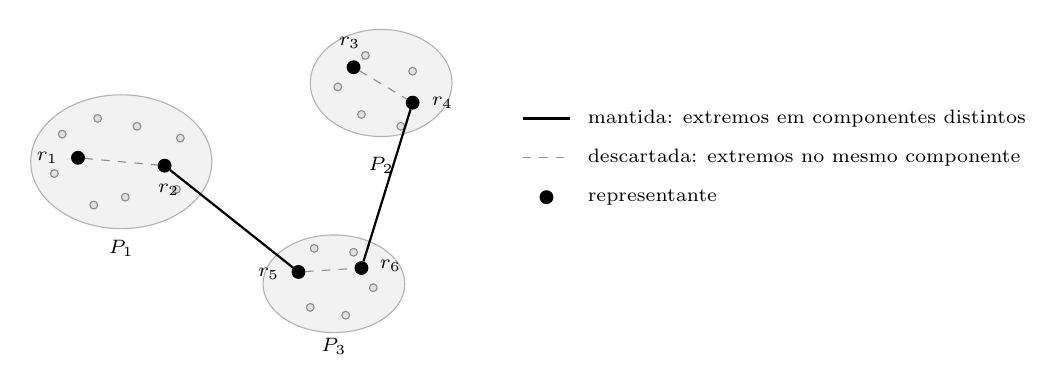
\begin{tikzpicture}[
  blob/.style={draw=black!30, fill=black!5},
  pt/.style={circle, draw=black!45, fill=black!12, inner sep=0pt, minimum size=2.8pt},
  rep/.style={circle, draw=black, fill=black, inner sep=0pt, minimum size=4.6pt},
  keep/.style={black, thick},
  drop/.style={black!45, dashed, thin},
  lb/.style={font=\scriptsize},
  cp/.style={font=\scriptsize}
]
% componentes
\draw[blob] (0,0) ellipse (1.15 and 0.85);
\draw[blob] (3.30,1.00) ellipse (0.90 and 0.68);
\draw[blob] (2.70,-1.55) ellipse (0.90 and 0.62);
\node[lb] at (0,-1.10) {$P_1$};
\node[lb] at (3.30,-0.05) {$P_2$};
\node[lb] at (2.70,-2.35) {$P_3$};
% pontos internos
\foreach \x/\y in {-0.75/0.35, -0.30/0.55, 0.20/0.45, 0.75/0.30, -0.85/-0.15,
                   0.05/-0.45, 0.70/-0.35, -0.35/-0.55}
   \node[pt] at (\x,\y) {};
\foreach \x/\y in {3.05/0.60, 3.55/0.45, 3.70/1.15, 3.10/1.35, 2.75/0.95}
   \node[pt] at (\x,\y) {};
\foreach \x/\y in {2.45/-1.10, 2.95/-1.15, 3.20/-1.60, 2.40/-1.85, 2.85/-1.95}
   \node[pt] at (\x,\y) {};
% representantes
\node[rep] (r1) at (-0.55, 0.05) {};
\node[rep] (r2) at ( 0.55,-0.05) {};
\node[rep] (r3) at ( 2.95, 1.20) {};
\node[rep] (r4) at ( 3.70, 0.75) {};
\node[rep] (r5) at ( 2.25,-1.40) {};
\node[rep] (r6) at ( 3.05,-1.35) {};
\node[lb, anchor=east]  at (-0.68, 0.05) {$r_1$};
\node[lb, anchor=north] at ( 0.60,-0.16) {$r_2$};
\node[lb, anchor=south] at ( 2.90, 1.32) {$r_3$};
\node[lb, anchor=west]  at ( 3.82, 0.75) {$r_4$};
\node[lb, anchor=east]  at ( 2.13,-1.42) {$r_5$};
\node[lb, anchor=west]  at ( 3.16,-1.32) {$r_6$};
% arvore geradora sobre os representantes
\draw[drop] (r1) -- (r2);
\draw[drop] (r3) -- (r4);
\draw[drop] (r5) -- (r6);
\draw[keep] (r2) -- (r5);
\draw[keep] (r6) -- (r4);
% legenda
\draw[keep] (5.10,0.55) -- (5.70,0.55);
\node[lb, anchor=west] at (5.80,0.55) {mantida: extremos em componentes distintos};
\draw[drop] (5.10,0.05) -- (5.70,0.05);
\node[lb, anchor=west] at (5.80,0.05) {descartada: extremos no mesmo componente};
\node[rep] at (5.40,-0.45) {};
\node[lb, anchor=west] at (5.80,-0.45) {representante};
\end{tikzpicture}\\
Fonte: Autoral.
\end{figure}

Ambos os mecanismos precisam saber a que componente pertence cada vértice, de modo que uma rotulação de componentes é calculada uma vez por atualização. Ela é uma passagem de união-busca sobre os arranjos de adjacência do \ac{k-NNG}, que percorre todos os vértices; adicionar as arestas de ponte à rotulação em seguida custa uma união adicional por ponte. O fato de a rotulação ser global levanta a pergunta óbvia de por que a pontuação anti-hub é necessária, se os componentes são conhecidos de qualquer forma. A resposta é que saber quais vértices pertencem a um componente não diz de qual deles uma ponte deve partir, e um componente pode conter milhões de vértices. Ligar componentes diretamente exigiria uma busca entre todos os pares de dois deles; a pontuação é o que reduz cada componente ao punhado de vértices de borda que vale a pena considerar, e a árvore geradora é então calculada sobre esse conjunto pequeno.\\

\subsection{O índice de hubness como observador\label{sec:hubindex}}

Duas propriedades da implementação merecem ser enunciadas. O índice de \textit{hubness} se acopla ao \ac{k-NNG} como um observador, de modo que toda aresta direcionada inserida ou removida atualiza um grau reverso em $O(1)$ e marca os vértices afetados; uma atualização repontua apenas a região afetada, em vez de todos os $n$ vértices.\\

Além disso, o índice mantém as próprias vizinhanças reversas, além dos graus reversos, o que torna exata a propagação da pontuação após uma atualização. Isso porque $\mathrm{score}(v)$ depende de $\mathrm{rd}(u)$ para $u \in \mathrm{NN}(v)$, de modo que os vértices que precisam ser repontuados quando o grau reverso de um vértice $u$ muda são aqueles que têm $u$ como vizinho, isto é, os vizinhos reversos de $u$. Essas mesmas listas são o que torna o grafo navegável para busca em feixe, propriedade que a construção não utiliza mas da qual o caminho de extensão da Seção \ref{sec:fut-streams} depende. O custo dessa escolha é um inteiro por aresta direcionada, e ela pode ser desativada, momento em que a propagação recai para uma aproximação sobre arestas diretas e a busca segue apenas arestas diretas.\\

% =====================================================================
\section{O algoritmo\label{sec:algorithm}}
% =====================================================================

O método é apresentado em duas rotinas, correspondentes às duas metades do \ac{CORE-SG}. O Algoritmo \ref{alg:knn} constrói o grafo de vizinhança por decomposição em instâncias, cobrindo as duas primeiras etapas da Figura \ref{fig:pipeline}. O Algoritmo \ref{alg:bridges} estima a metade de árvore geradora, cobrindo as duas últimas. As duas rotinas não compartilham estado além do \ac{k-NNG} concluído, o que é a razão de serem descritas e medidas separadamente.\\

A extração da $\mathrm{MST}_{\mpts}$ para um valor específico do parâmetro é a consulta, e não a construção: ela consiste em repesar com $\mrd^{\mpts}$ a união das arestas produzidas pelas duas rotinas e executar um algoritmo de árvore geradora mínima sobre elas.\\

\begin{algorithm}[htb!]
\caption{\label{alg:knn} O grafo de vizinhança, a partir de instâncias independentes}
\begin{algorithmic}[1]
\REQUIRE conjunto $X$ com $|X| = n$; tamanho de vizinhança $\kmax$; quantidade de instâncias $m$; fração de sobreposição $\omega$; taxa de parada $\delta$; rodadas de reparo $r$
\ENSURE grafo $G$ de $\kmax$ vizinhos mais próximos sobre $X$
\STATE corte uma permutação aleatória de $X$ em blocos $B_1, \dots, B_m$
\FOR{$i \leftarrow 1$ \TO $m$}
    \COMMENT{independentes; qualquer acelerador}
    \STATE $S_i \leftarrow \omega|B_i|$ pontos sorteados uniformemente em $X \setminus B_i$
    \STATE $V_i \leftarrow B_i \cup S_i$
    \STATE $H_i \leftarrow \textsc{NNDescent}(V_i, \kmax)$, parando quando uma rodada produzir menos de $\delta\kmax|V_i|$ atualizações
\ENDFOR
\STATE $G \leftarrow$ listas vazias de $\kmax$ melhores sobre $X$
\FOR{$i \leftarrow 1$ \TO $m$}
    \COMMENT{mesclagem; independente da ordem}
    \FORALL{$v \in B_i$ e $(u, w) \in H_i[v]$}
        \STATE ofereça $(u, w)$ a $G[v]$, que retém os $\kmax$ menores
    \ENDFOR
\ENDFOR
\IF{$m > 1$}
    \STATE $G \leftarrow \textsc{NNDescent}(G, \kmax)$ por $r$ rodadas
    \COMMENT{passo de reparo, na \ac{CPU}}
\ENDIF
\RETURN $G$
\end{algorithmic}
\end{algorithm}

\begin{algorithm}[htb!]
\caption{\label{alg:bridges} A metade de árvore geradora, estimada por anti-hubs}
\begin{algorithmic}[1]
\REQUIRE grafo $G$ com conjunto de arestas não direcionadas $E$; dimensionalidade $d$; multiplicador $\alpha$; cota de seleção $q$; representantes por componente $\rho$
\ENSURE conjunto de arestas de ponte $\mathcal{B}$
\FORALL{$v \in V(G)$}
    \STATE $\mathrm{rd}(v) \leftarrow |\{u : v \in \mathrm{NN}(u)\}|$
    \COMMENT{grau reverso, Eq.~\eqref{eq:rd}}
\ENDFOR
\FORALL{$v \in V(G)$}
    \STATE $\mathrm{score}(v) \leftarrow \mathrm{rd}(v) \big/ \big( |\mathrm{NN}(v)|^{-1}\textstyle\sum_{u \in \mathrm{NN}(v)} \mathrm{rd}(u) \big)$
    \COMMENT{Eq.~\eqref{eq:score}}
\ENDFOR
\STATE $\mathcal{C} \leftarrow \textsc{ComponentesConexos}(G)$
\COMMENT{união-busca sobre a adjacência}
\STATE $A \leftarrow$ os $\lceil \alpha d \ln|E| \rceil$ vértices menores na ordem $(\mathrm{score}, \mathrm{rd}, \mathrm{id})$
\FORALL{$c \in \mathcal{C}$}
    \STATE $A \leftarrow A \cup \{$os $q$ vértices de $c$ menores nessa ordem$\}$
    \COMMENT{cota por componente}
\ENDFOR
\STATE $\mathcal{B} \leftarrow \textsc{MSTExata}(A)$ sob $\mrd^{\kmax}$, com cada aresta armazenada por sua distância de base
\STATE $\mathcal{C}' \leftarrow \textsc{ComponentesConexos}(G \cup \mathcal{B})$
\IF{$|\mathcal{C}'| > 1$}
    \COMMENT{a estimativa deixou uma floresta}
    \STATE $D \leftarrow \bigcup_{c \in \mathcal{C}'} \{$os $\rho$ vértices de menor pontuação de $c\}$
    \STATE $T \leftarrow \textsc{MSTExata}(D)$ sob $\mrd^{\kmax}$
    \STATE $\mathcal{B} \leftarrow \mathcal{B} \cup \{e \in T : \text{os extremos de } e \text{ estão em componentes distintos de } \mathcal{C}'\}$
\ENDIF
\RETURN $\mathcal{B}$
\end{algorithmic}
\end{algorithm}

Duas observações sobre o Algoritmo \ref{alg:knn} merecem registro, porque correspondem a decisões que poderiam ser tomadas de outra forma.\\

A primeira é que a condição da linha que precede o passo de reparo não é uma otimização, e sim a definição do caso base. Em $m = 1$ não há partição, nenhum par deixa de ser comparado, e o resultado da descida é o grafo final; executar um reparo ali equivaleria a mais rodadas de NN-Descent sobre o mesmo grafo, que é uma escolha distinta da adotada aqui.\\

A segunda é que a mesclagem percorre apenas $v \in B_i$, deixando de fora $v \in V_i$. As vizinhanças descobertas para os pontos de sobreposição são usadas durante a descida, pois é através delas que os pares que cruzam fronteiras são comparados; elas não são, porém, oferecidas à mesclagem por uma instância que não possui esses pontos. Cada vértice é oferecido à lista global pela instância que o possui, o que mantém o custo da mesclagem em $O(n\kmax)$ independentemente de $\omega$.\\

Sobre o Algoritmo \ref{alg:bridges}, a ordem de seleção da linha correspondente é um critério total e determinístico, por pontuação, depois grau reverso, depois identificador. O desempate explícito não é cosmético: sem ele, duas execuções sobre o mesmo grafo selecionariam conjuntos de anti-hubs distintos sempre que houvesse empates de pontuação, que são frequentes em componentes de densidade uniforme, e o método deixaria de ser reprodutível.\\

% =====================================================================
\section{Implementação e execução em múltiplos aceleradores\label{sec:implementation}}
% =====================================================================

O método foi implementado em C++17, com os núcleos de descida e de cálculo de distâncias em \ac{CUDA}. Existe também um ambiente de execução em \ac{CPU}, usado para verificar que as afirmações do trabalho não dependem do acelerador, e para os casos em que nenhum dispositivo está disponível. A concordância entre os dois ambientes é reportada na Seção \ref{sec:res-parity}.\\

O esquema de execução multi-\ac{GPU} decorre diretamente da decomposição em instâncias. Cada instância é um problema autocontido, e por isso pode ser transferida a um dispositivo, executada até a convergência e ter seu resultado recolhido sem qualquer comunicação com as demais. As instâncias são enfileiradas em uma fila de trabalho e atribuídas ao próximo dispositivo livre. A mesclagem descrita na Seção \ref{sec:merge}, por ser comutativa, associativa e idempotente, aceita os resultados na ordem em que chegam.\\

Esse desenho tem duas consequências, ambas verificadas experimentalmente no Capítulo \ref{cha:results}. A primeira é que a memória por dispositivo é determinada pela quantidade de instâncias e pela fração de sobreposição, independentemente da quantidade de dispositivos: dividir o trabalho em mais instâncias reduz o consumo por dispositivo, ao passo que adicionar dispositivos não o altera. A resposta a um conjunto de dados que não cabe é, portanto, reparticionar sobre o mesmo hardware. A segunda é que o paralelismo disponível é limitado pela quantidade de instâncias: com uma única instância, adicionar dispositivos não produz aceleração alguma, independentemente de quantos estejam presentes.\\

Quando uma instância não cabe no dispositivo a que foi atribuída, a implementação recorre a um mecanismo de reserva que a executa na \ac{CPU} em vez de falhar. Esse mecanismo existe para que uma configuração mal dimensionada produza um resultado lento em vez de um erro, mas sua ativação é contabilizada e reportada, porque uma execução em que instâncias caíram para a \ac{CPU} não mede o que o experimento pretendia medir.\\

As etapas globais da construção (a mesclagem, o passo de reparo, a árvore geradora das pontes e a rotulação de componentes) são executadas em uma \ac{CPU} multithread. Que o passo de reparo esteja entre elas é a limitação central do método, discutida no Capítulo \ref{cha:discussion}.\\

% =====================================================================
\section{Protocolo experimental\label{sec:protocol}}
% =====================================================================

\subsection{Referência exata\label{sec:ground-truth}}

A qualidade é medida contra computações exatas e nunca contra rótulos de classe. A afirmação sob teste é que uma aproximação corresponde ao objeto que ela aproxima. Pontuar contra rótulos de classe mediria, em vez disso, se o \ac{HDBSCAN*} é adequado a um dado conjunto, o que é um problema fora do escopo deste trabalho.\\

Duas referências exatas são usadas, uma por pergunta. A estimativa de pontes é pontuada contra o \ac{CORE-SG} exato, ou seja, um \ac{k-NNG} exato por força bruta somado a uma $\mathrm{MST}_{\kmax}$ exata, já que a pergunta é se a estimativa corresponde à árvore geradora que ela substitui. A revocação da vizinhança é pontuada contra um \ac{k-NNG} exato por força bruta sobre os mesmos pontos.\\

Acima de $n = 2 \times 10^5$ a referência exaustiva, que custa $O(n^2 d)$, torna-se inviável e é substituída por uma estimativa amostrada: 2.000 vértices de consulta sorteados uniformemente, cada um pontuado exatamente contra todos os pontos, ao custo de $O(q n d)$ para $q$ consultas. Em revocação próxima de 0,98, o erro padrão da média amostral fica abaixo de 0,003, o que é uma ordem de grandeza menor que as diferenças que o Capítulo \ref{cha:results} discute.\\

Uma comparação usa a construção de instância única como referência em lugar das anteriores, por uma razão que constitui um desvio do critério acima. O efeito sob teste ali é o custo do particionamento: o que muda no resultado quando um conjunto é cortado em $m$ blocos em vez de descido como um só. Um \ac{CORE-SG} exato não isola isso, porque difere de qualquer um dos dois braços da comparação em dois aspectos simultaneamente: a partição e o fato de a metade de vizinhança ser exata. Uma construção de instância única difere apenas na partição.\\

Comparar dois \ac{CORE-SG}s construídos independentemente carrega, contudo, uma ressalva, que é a razão pela qual essa referência é usada para algumas grandezas e não para outras. Ambos os lados constroem seu grafo de vizinhança por uma descida aleatorizada, e duas execuções dessa descida sobre os mesmos pontos não concordam aresta a aresta. Sobre as grandezas que agregam o grafo inteiro, como o agrupamento plano e o peso total da árvore geradora, essa discordância é pequena diante do efeito sob medição. Sobre as pontes ela não é: o conjunto de pontes é escolhido a partir de uma pontuação calculada sobre a metade de vizinhança, de modo que dois braços com metades de vizinhança distintas selecionam anti-hubs parcialmente distintos, e a razão de peso resultante já foi observada abaixo de 1, o que é impossível para uma aproximação genuína e indica que a comparação está medindo a grandeza errada. A qualidade das pontes é, por isso, medida apenas onde ambos os braços compartilham uma metade de vizinhança exata.\\

\subsection{Métricas\label{sec:metrics}}

São reportadas cinco métricas principais.\\

A revocação do \ac{k-NN} é a fração dos verdadeiros $k$ vizinhos mais próximos que estão presentes no grafo aproximado. Ela mede diretamente a qualidade do grafo de vizinhança e é a grandeza que a construção aproximada degrada. É a métrica padrão da literatura de busca aproximada de vizinhos \cite{annbench}, o que torna os valores aqui reportados comparáveis aos daquele campo.\\

A razão de peso da \ac{MST} é o peso total da árvore geradora aproximada dividido pelo peso total da exata. Ela é uma afirmação sobre o dendrograma, acima de um simples total, porque os pesos ordenados da \ac{MST} são as alturas de fusão da ligação simples. Uma razão de 1 significa que as duas árvores induzem exatamente a mesma sequência de fusões.\\

A maior diferença pontual entre os perfis de peso ordenados é o máximo, sobre as posições da ordenação, do valor absoluto da diferença entre o $i$-ésimo peso de uma árvore e o $i$-ésimo peso da outra. Ela enuncia quanto se deslocou a fusão mais afetada, ao passo que a razão de peso agrega o deslocamento de todas elas. Uma razão próxima de 1 acompanhada de uma diferença pontual grande indicaria que poucas fusões se moveram muito, o que altera a hierarquia mesmo sem alterar o total.\\

O número de arestas divergentes é a quantidade de arestas de uma das árvores que não estão presentes na outra, sobre as $n-1$ arestas de uma árvore geradora. Um valor zero estabelece que as duas árvores são idênticas, o que nenhuma métrica agregada consegue estabelecer.\\

O \ac{ARI} do DBSCAN* \cite{ari} é o índice Rand ajustado entre os agrupamentos planos cortados de ambas as árvores em um limiar comum. O índice Rand mede a fração de pares de objetos sobre os quais duas partições concordam, e sua forma ajustada corrige o valor esperado sob atribuição aleatória, de modo que 1 indica partições idênticas e 0 indica concordância equivalente ao acaso. A correção por acaso é o que torna o índice interpretável quando as partições comparadas têm números distintos de grupos, situação em que a forma não corrigida cresce com a quantidade de grupos; a mesma correção se aplica às medidas de concordância derivadas da teoria da informação \cite{ami}, cujo uso aqui seria redundante, já que as partições comparadas provêm do mesmo corte sobre árvores quase idênticas.\\

As duas últimas respondem a perguntas diferentes e ambas são necessárias: a contagem de arestas divergentes estabelece se houve diferença, e a razão de peso estabelece se essa diferença custou alguma coisa. O \ac{ARI} é a mais fraca das quatro sempre que as duas árvores são extraídas de grafos que compartilham um subgrafo comum, pela razão exposta na Seção \ref{sec:res-bridges}.\\

Três grandezas adicionais precisam de definição.\\

A contagem de componentes do \ac{k-NNG} antes do reparo é o número de componentes conexos em que o grafo de vizinhança se divide por conta própria, sem nenhuma ponte adicionada e sem reparo aplicado. Ela enuncia quanto trabalho as pontes têm a fazer, e um valor de 1 significa que elas não têm nenhum. Essa grandeza precisou ser corrigida durante a pesquisa, e o registro da correção importa porque números anteriores dependiam dela: em sua primeira forma, ela era coletada depois de as arestas de ponte serem incorporadas à rotulação de componentes, e por isso lia 1 em toda execução, houvessem as pontes funcionado ou não. A forma reportada neste trabalho é coletada antes de qualquer ponte ser adicionada, e por isso pode assumir valores maiores que 1, como ocorre na Seção \ref{sec:res-quota}.\\

O tempo de relógio decomposto por fase separa uma atualização em busca de semeadura, descida das instâncias, mesclagem, refinamento restrito, atualização de \textit{hubness}, árvore geradora das pontes e passagem de conectividade, de modo que a porção paralela possa ser separada do restante sequencial. É dessa decomposição que se extrai a fração paralela $f$ usada na análise de escalabilidade.\\

A maior instância residente é a memória de dispositivo que a maior instância de uma construção exigiu. É a grandeza que decide se uma configuração cabe em um dado acelerador, e portanto a que responde diretamente ao problema da Seção \ref{sec:problem-scale}. Ela é reportada em bytes efetivamente alocados, de modo que a Equação \eqref{eq:devicecost} possa ser confrontada com a medição.\\

A fração paralela $f$ é o tempo da fase de instâncias dividido pelo tempo total da construção. É a parcela do trabalho que executa nos aceleradores e que, portanto, se beneficia de acrescentá-los; pela lei de Amdahl \cite{amdahl}, ela limita superiormente a aceleração alcançável por qualquer quantidade de dispositivos. Reportá-la ao lado do tempo total é o que distingue uma construção que não acelerou por estar mal dimensionada de uma que não acelerou por ser dominada por fases sequenciais.\\

Uma métrica é deliberadamente omitida: a sobreposição de arestas entre duas \ac{MST}s do mesmo grafo. Todas as \ac{MST}s de um grafo compartilham o mesmo multiconjunto de pesos, e para qualquer limiar os componentes do conjunto de arestas abaixo dele dependem do grafo e não de qual \ac{MST} foi extraída, de modo que duas \ac{MST}s diferentes induzem hierarquias de ligação simples muito semelhantes. Medido neste sistema, a sobreposição cai de 0,99 para 0,19 conforme $\mpts$ sobe de 1 para 32 enquanto o \ac{ARI} permanece exatamente 1,0000, porque aumentar $\mpts$ achata a paisagem de \textit{mutual reachability} em platôs de pesos empatados e qualquer critério de desempate produz uma árvore diferente e igualmente ótima.\\

A contagem de arestas divergentes definida acima não incorre nessa objeção, e a distinção importa porque as duas grandezas se parecem. Ela é aplicada apenas quando uma das árvores é extraída de um subgrafo da outra, caso da ablação da Seção \ref{sec:res-connectivity}. Nesse regime, uma aresta divergente não pode ser um artefato de desempate: a árvore sobre o subgrafo nunca pode ser mais leve que a árvore sobre o grafo completo, de modo que qualquer divergência corresponde a um desvio que o subgrafo obrigou, e a razão de peso mede exatamente o preço desse desvio.\\

\subsection{Conjuntos de dados\label{sec:datasets}}

A Tabela \ref{tab:datasets} lista as três famílias utilizadas, mais uma família escala, empregada apenas na Seção \ref{sec:res-scale} e na sondagem de capacidade de instância única. Os conjuntos de escala são sintéticos, gerados em $d = 32$ com dimensionalidade intrínseca 8, 200 grupos e separação fixa, em tamanhos de $10^7$ a $5 \times 10^7$ pontos; eles existem porque nenhum conjunto público ao qual tivemos acesso alcança essas magnitudes, e a afirmação principal do trabalho trata do regime em que a construção não decomposta deixa de caber no dispositivo.\\

Os conjuntos real-paper reproduzem as receitas de preparação do trabalho original do \ac{CORE-SG} \cite{core-sg} para fins de comparabilidade, usando FMA \cite{fma} e 20 Newsgroups \cite{newsgroups}. Os conjuntos real-scale exercitam escala, alta dimensionalidade e uma métrica não euclidiana: SIFT1M e GIST1M \cite{sift_gist}, e GloVe \cite{glove} sob distância do cosseno. Os conjuntos manifold são sintéticos, gerados em baixa dimensionalidade e rotacionados para uma alta por um mapa ortonormal aleatório, o que preserva exatamente toda distância entre pares, de modo que a estrutura de componentes e sua separação permanecem intactas enquanto a dimensionalidade ambiente sobe e a dimensionalidade intrínseca é conhecida por construção.\\

A família \textit{manifold} existe por causa de uma constatação reportada na Seção \ref{sec:res-connectivity}: nenhum conjunto de dados real examinado produz um \ac{k-NNG} fragmentado, de modo que nenhum deles é capaz de exercitar as pontes.\\

\begin{table}[htb!]
\caption{\label{tab:datasets} Conjuntos de dados. A coluna ``comp.'' é o número de componentes do \ac{k-NNG} sozinho no $\kmax$ de operação, medido com um \ac{k-NNG} \textit{exato} para os conjuntos de $n = 4.000$, onde a referência exata é viável, e com o grafo \textit{aproximado} em $n$ completo para os demais.}
\centering
\footnotesize
\begin{tabular}{@{}llrrrr@{}}
\toprule
família & conjunto & $n$ & $d$ & $\kmax$ & comp. \\
\midrule
real-paper & \texttt{fma\_chroma}   & 106.574 & 84   & 32 & 1 \\
           & \texttt{fma\_mfcc}     & 106.574 & 140  & 32 & 1 \\
           & \texttt{20ng\_tfidf}   & 10.969  & 1000 & 24 & 1 \\
           & \texttt{20ng\_pca500}  & 10.969  & 500  & 24 & 1 \\
\midrule
real-scale & \texttt{sift1m}        & 200.000 & 128  & 32 & 1 \\
           & \texttt{gist1m}        & 100.000 & 960  & 32 & 1 \\
           & \texttt{glove100}      & 200.000 & 100  & 32 & 1 \\
\midrule
manifold   & \texttt{manifold\_exact} & 4.000   & 128 & 24 & 16 \\
           & \texttt{manifold\_c8}    & 4.000   & 128 & 24 & 8  \\
           & \texttt{manifold\_c24}   & 4.000   & 64  & 24 & 24 \\
           & \texttt{manifold\_c32}   & 4.000   & 128 & 16 & 32 \\
           & \texttt{manifold\_mid}   & 100.000 & 128 & 24 & 132 \\
           & \texttt{manifold\_wide}  & 100.000 & 256 & 24 & 271 \\
\midrule
escala     & \texttt{scale10000000} & 10.000.000 & 32 & 32 & n/a \\
           & \texttt{scale20000000} & 20.000.000 & 32 & 32 & n/a \\
           & \texttt{scale30000000} & 30.000.000 & 32 & 32 & n/a \\
           & \texttt{scale40000000} & 40.000.000 & 32 & 32 & n/a \\
           & \texttt{scale50000000} & 50.000.000 & 32 & 32 & n/a \\
\bottomrule
\end{tabular}\\
Fonte: Autoral.
\end{table}

A preparação do conjunto 20 Newsgroups afeta a validade de qualquer medição sobre ele. A receita do trabalho original, que seleciona os 1000 termos de maior TF-IDF, deixa aproximadamente 3\% dos documentos com um vetor inteiramente nulo. Como a vetorização normaliza os vetores, todo documento real fica a distância exatamente 1,0 de todo documento vazio, o que é mais próximo que seus vizinhos genuínos. A vizinhança de um documento típico torna-se, então, composta por documentos vazios a distâncias idênticas, o que achata as \textit{core distances} entre valores de $\mpts$ e degrada a própria estrutura de densidade, além do estimador de dimensionalidade. Os documentos vazios são, por isso, descartados na preparação usada aqui.\\

\subsection{Linhas de base\label{sec:baselines}}

A linha de base interna principal é a construção de instância única, isto é, $m = 1$. Ela não realiza partição e, por consequência, nenhum reparo, e é a configuração a que uma construção centralizada corresponde. Toda contagem de instâncias é cobrada contra ela sobre os mesmos dados, a mesma semente e a mesma quantidade de dispositivos, de modo que a razão isole o custo da decomposição de qualquer outra diferença.\\

A linha de base externa é a biblioteca NVIDIA cuML \cite{cuml}, que fornece uma implementação do \ac{HDBSCAN*} em \ac{GPU}. O tempo de relógio é comparável nesse caso porque ambas as implementações são \ac{CUDA} e executam no mesmo dispositivo. A cuML serve um valor de $\mpts$ por ajuste, de modo que a propriedade de múltiplos $\mpts$ do \ac{CORE-SG} não tem equivalente naquela implementação e é reportada separadamente.\\

A restrição de comparabilidade enunciada no parágrafo anterior governa quais comparações este capítulo autoriza. \citeonline{blackart} demonstram que tempos de execução medidos entre implementações distintas de um mesmo algoritmo variam por ordens de grandeza, e que comparações entre algoritmos conduzidas por tempo de relógio frequentemente medem a qualidade das implementações. A consequência metodológica adotada aqui é que o tempo de relógio só é comparado quando as implementações comparadas compartilham linguagem, modelo de execução e dispositivo, o que vale entre as configurações deste trabalho e entre elas e a cuML. Contra os demais métodos da literatura, a comparação é de propriedades estruturais, como residência de memória por dispositivo e faixa de $\mpts$ atendida.\\

Os candidatos considerados e excluídos atacam um eixo distinto. O I-HASTREAM \cite{ihastream} mantém uma hierarquia sobre microgrupos, e Data Bubbles \cite{databubbles} e métodos derivados do BIRCH \cite{birch} agrupam sobre sumários; pontuá-los contra uma referência no nível dos pontos confundiria o erro introduzido pela sumarização com o erro introduzido pela decomposição. O FISHDBC \cite{fishdbc} mantém uma estrutura sob inserção e serve um único $\mpts$. O \ac{HDBSCAN*} sobre MapReduce \cite{mrhdbscan}, o \ac{HDBSCAN*} acelerado \cite{acceleratedhdbscan} e o esquema híbrido de \ac{CPU} e \ac{GPU} \cite{bpshdbscan} distribuem um agrupamento de parâmetro único, em lugar de uma estrutura que sirva a uma faixa de $\mpts$.\\

Não se compara, tampouco, contra bibliotecas de construção aproximada de \ac{k-NNG}, porque este trabalho não afirma construir um \ac{k-NNG} mais rápido: ele usa o NN-Descent \cite{nndescent, dynamic_nndescent} e contribui com uma decomposição da construção. Uma verificação de revocação contra força bruta estabelece que o grafo produzido é sólido, que é a propriedade de que o argumento precisa.\\

Nenhum método publicado constrói, distribuído entre múltiplos aceleradores, uma estrutura que sirva a uma faixa de valores de $\mpts$, razão pela qual a comparação principal é feita contra a construção de instância única.\\

\subsection{Hardware e procedimento\label{sec:hardware}}

As medições foram tomadas em um agregado de 4 \ac{GPU}s RTX 2080 SUPER (arquitetura sm\_75, 8\,GB de memória por dispositivo, \ac{CUDA} 12.9), salvo indicação em contrário; um subconjunto foi tomado em uma única RTX 4070 Ti SUPER e está rotulado como tal. As figuras de qualidade, ou seja, contagens de componentes, revocação, \ac{ARI} e razões entre tempos medidos na mesma máquina, são independentes do hardware; as figuras absolutas de tempo de relógio não são, e nunca são agregadas entre máquinas.\\

Todo experimento usa múltiplas sementes aleatórias, porque o NN-Descent é aleatorizado e seu cache de vizinhos reversos é deliberadamente tolerante a corridas entre threads. Experimentos que mantêm o \ac{k-NNG} exato são determinísticos e usam 2 sementes, o que foi verificado observando um desvio padrão de exatamente zero em 5 sementes.\\

\subsection{Infraestrutura\label{sec:infrastructure}}

A Universidade Federal de São Carlos, campus São Carlos, por meio do laboratório MIDAS (Mineração de Dados e Aplicações), proporciona o espaço físico e os equipamentos necessários ao desenvolvimento do projeto, incluindo o agregado de aceleradores usado nas medições. A instituição, em parceria com repositórios de artigos e trabalhos acadêmicos, permite o acesso às referências bibliográficas necessárias à pesquisa, além daquelas acessadas pela internet.\\
